\documentclass[10pt, final]{article}
% \documentclass[10pt,technote]{IEEEtran}
\usepackage[a4paper,width=185mm,top=20mm,bottom=20mm]{geometry}
\usepackage{pythonhighlight}
\usepackage{url}
\usepackage{lipsum}
\usepackage{amsmath, amssymb}
\usepackage{multicol}
\setlength{\columnsep}{1cm}
\usepackage{graphicx}
\graphicspath{{../results/}{../immagini/}}
\DeclareGraphicsExtensions{.png, .pdf}
\usepackage{wrapfig}
\usepackage[font=small,labelfont=bf]{caption}
\usepackage{setspace}
\usepackage{caption}
\usepackage{subcaption}
\usepackage{wrapfig}
\usepackage{float}
\usepackage{xcolor}
\usepackage[tikz]{mdframed}
\usepackage{colortbl}
\usepackage{MnSymbol}
\usepackage[T1]{fontenc}
\usepackage{ascii}
\usepackage{listings}

\lstset{prebreak=\raisebox{0ex}[0ex][0ex]
        {\ensuremath{\rhookswarrow}}}
\lstset{postbreak=\raisebox{0ex}[0ex][0ex]
        {\ensuremath{\rcurvearrowse\space}}}
\lstset{breaklines=true, breakatwhitespace=true}
\lstset{numbers=left, numberstyle=\scriptsize}
\DeclareMathOperator{\E}{\mathbb{E}}

\UseRawInputEncoding %%%%%%%%%%%%%%%%%%%%%%%%%OCCHIOOOOOO
\definecolor{forestgreen}{rgb}{0.0, 0.27, 0.13}
%%
%% Julia definition (c) 2014 Jubobs
%%
\lstdefinelanguage{Julia}%
  {morekeywords={abstract,break,case,catch,const,continue,do,else,elseif,%
      end,export,false,for,function,immutable,import,importall,if,in,%
      macro,module,otherwise,quote,return,switch,true,try,type,typealias,%
      using,while},%
   sensitive=true,%
   alsoother={\$},%
   morecomment=[l]\#,%
   morecomment=[n]{\#=}{=\#},%
   morestring=[s]{"}{"},%
   morestring=[m]{'}{'},%
}[keywords,comments,strings]%

\lstset{%
    language         = Julia,
    basicstyle       = \ttfamily,
    keywordstyle     = \bfseries\color{blue},
    stringstyle      = \color{magenta},
    commentstyle     = \color{forestgreen},
    showstringspaces = false,
}


\definecolor{airforceblue}{rgb}{0.36, 0.54, 0.66}
\mdfsetup{
middlelinecolor=airforceblue,%
middlelinewidth=0.2pt,%
roundcorner=5pt}
\setlength{\abovedisplayskip}{3pt}
\setlength{\belowdisplayskip}{3pt}

\renewcommand{\baselinestretch}{1}

\title{\textsc{Report 2 - Grangier-Roger-Aspect experiment analysis}}
\author{Francesco Lorenzi,      October-November 2020}
\date{}
\begin{document}
\maketitle
\vspace{-25pt}

\begin{center}
	\rule[0pt]{400pt}{0.5pt}
\end{center}
\vspace{-15pt}

\begin{multicols}{2}
\subsubsection*{Summary}
The purpose of this report is twofold: in a first part a statistical analysis will be carried out on a dataset collected from an experimental setup based on Grangier-Roger-Aspect experiment \cite{grangier}. 

In a second part, an application of photon arrival statistics is shown: using a dataset from coherent light photon detection, random integers are generated and analyzed using various visual techniques.

\section{Photon indivisibility experiment}
The experiment developed by P. Grangier, G. Roger and A. Aspect in 1986 consist in verifying, by using statistical methods on photomultipliers hits, that a single  photon, after impinging on a beam splitter, cannot be effectively divided, and preserves its unity. The statistical outcome is expressed in terms of \emph{correlation} between photodetector events in the transmitted and reflected branch: the result highlight a very strong \emph{anticorrelation} between these events.

From the theoretical point of view, this experiment confirms the quanized nature of radiation, as the classical model for photodetection, which predicts correlation between detection along the two branches, is completely contradicted by the data.
\subsection*{Experimental and statistical setup}
Even if the description of the experiment with a single beam splitter and two detectors is straightfoward, an additional technique is needed to prevent detector noise from making the data unintelligible.
So instead of a single source, a source which emits photon \emph{in couples} is used, one is sent to a separate detector, and the other is sent to the setup described before. In that way the first photon triggers a \emph{gate} signal that validate counts from the other detectors. Assuming a low rate emission from the source with respect to dark count rate of photodiodes, with that technique the noise is greatly reduced.

Altought in the original experiment this feature was hardwired with electronics, in our setup all events are collected regardless of their validation, and the \emph{gate} signal is to be applied separately in post-processing.

The optical bench setup is shown in Figure \ref{our}: all the pulses from the photodiodes $PD_g, PD_t, PD_r$ are collected by a time-tagger on a common time scale in three different channels, respectively called \emph{gate (G)} channel, \emph{transmitted (T)} channel and \emph{reflected (R)} channel.


\begin{mdframed}
    \begin{figure}[H]
        \begin{subfigure}{\textwidth}
            \centering
            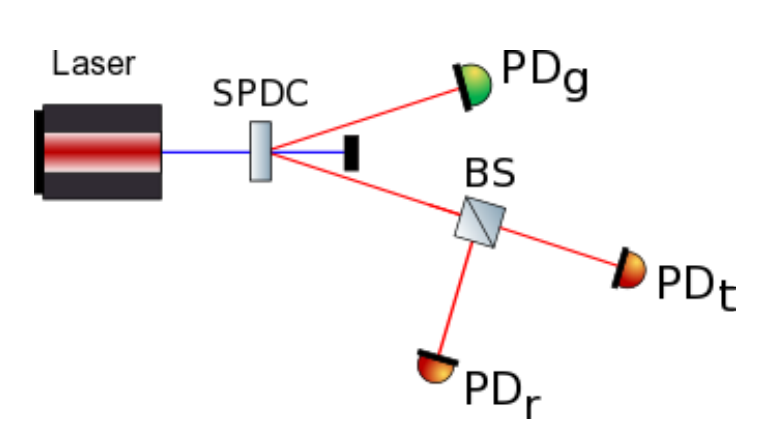
\includegraphics[width = 0.9\textwidth]{../images/our_setup.png}
            \caption{Actual setup}
            \label{our}
        \end{subfigure}

        \begin{subfigure}{\textwidth}
            \centering
            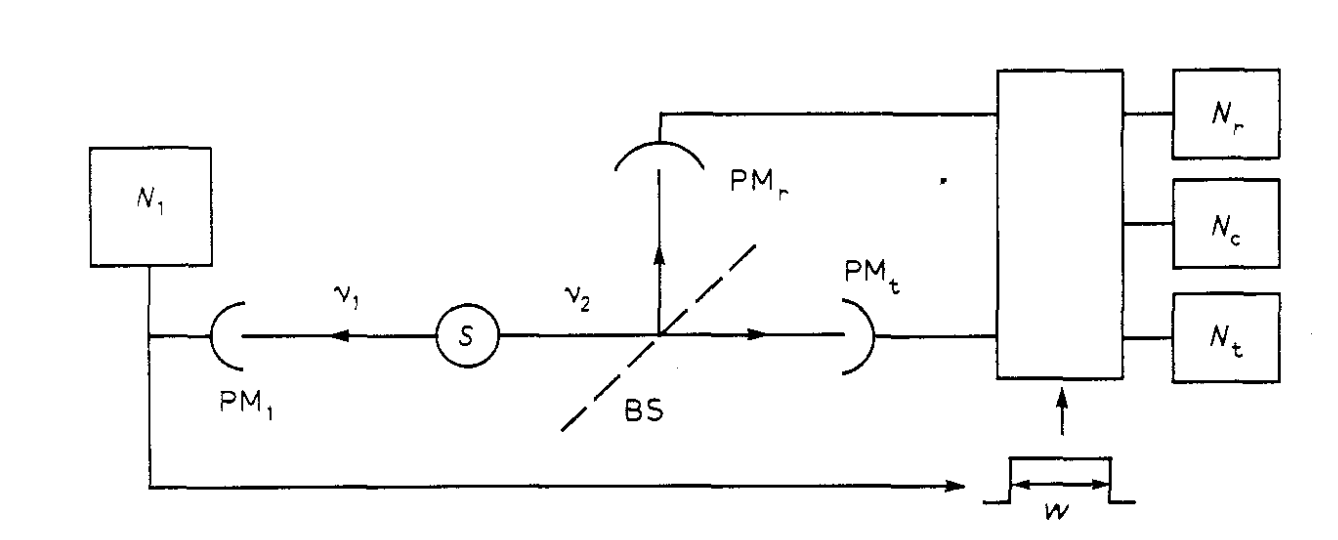
\includegraphics[width = \textwidth]{../images/original.png}
            \caption{Original setup}
        \end{subfigure}
        \caption{Experimental setup scheme}
    \end{figure}
\end{mdframed}
For every gate event, there is a constant probability $p_r$ and $p_t$ to have an event respectively in the $R$ and $T$ channels, within the temporal window of the gate function. 

In fact, we can define two Bernoulli random variables $X_r \sim B(p_r)$ and $X_t \sim B(p_t)$ which represents the result of measurement associated with each gate event. In this sense all the data collected can be represented as a stochastic process of i.i.d. variables. Each measurement will be called a \emph{double} coincidence if only one of the two realizations is $1$, and \emph{triple} coincidence if they are both $1$. 
If we call the probability of a triple coincidence $p_c$, it can't be assessed without knowing the correlation between the two variables, as the corresponding Bernoulli random variable is the product $X_r X_t$.

The physical problem is addressed by observing the correlation between the random variables, using the following definition of correlation coefficient: 
\begin{equation*}
    \alpha = \frac{p_c}{p_r p_t} = \frac{\E[X_r X_t]}{\E[X_r]\E[X_t]}.
\end{equation*}
If $\alpha > 1$ the variables are \emph{correlated}, and the classical model is confirmed, indeed if $\alpha < 1$ the variables are \emph{anticorrelated}, and the classical model is rejected in favour of the quantum model. This follows naturally from the concept of a photon indivisibility: if the photon can't be splitted we expect to never find triple coincidences.
Needless to say, we can only have an estimate of this parameter from experimental data: this is carried out as usual extracting a sample mean estimate using the following estimator: if $N_1$ is the number of valid gate events (associated with $R$ or $T$ events),
\begin{equation*}
    \hat{\alpha} = \frac{\hat{p_c}}{\hat{p_r} \hat{p_t}} = \frac{N_1 \sum_{i=1}^{N_1} X_r X_t}{\sum_{i=1}^{N_1} X_r\sum_{i=1}^{N_1} X_t},
\end{equation*}
Further comments on this estimator will be presented in the interpretation of result section.
\subsection*{Analysis}
As anticipated, before counting double and triple coincidences, a pre-processing step is necessary to remove noise. First of all, we reject events on the same channel which are distanced by less than $3900$ machine time units, or $MTU$ (defined by $1 MTU = 80.955 ps$). In fact, events whose difference in time is less than $\approx 0.315 \mu s$ could be \emph{afterpulses}, artifacts of the detection devices. After this passage the interarrival time of the three channels is plotted in Figure \ref{exps}, from which we can confirm that the light used is of coherent type, as it follows a Poisson arrival statistics.
\begin{mdframed}
    \begin{figure}[H]
        \centering
        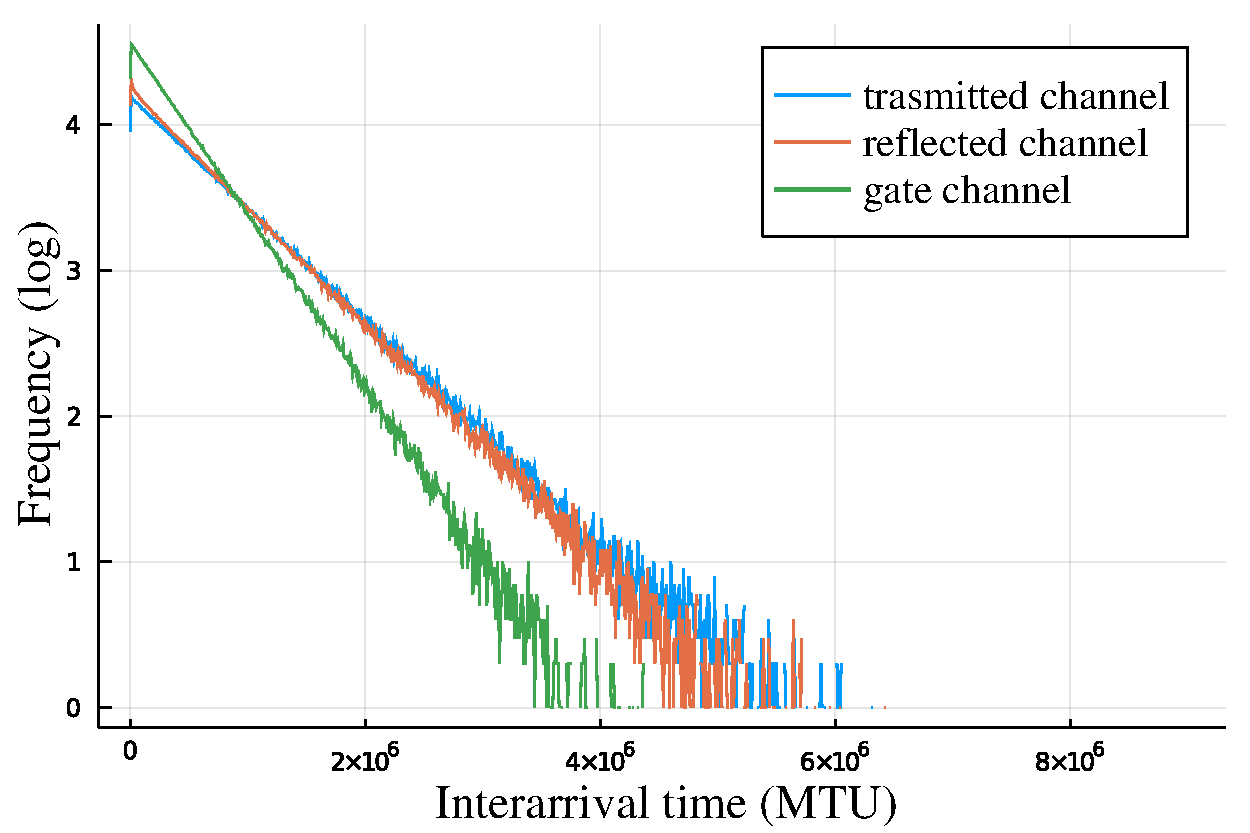
\includegraphics[width = \textwidth]{../images/single_chan.pdf}
        \caption{Single channel click frequencies}
        \label{exps}
    \end{figure}
\end{mdframed}

In a second step, we must filter the data with a suitable \emph{gate} function, which will be triggered by the events on the gate channel, and will detect events from the other channels which are included in a well defined \emph{window}. 

In order to build a correct gate window, we notice that the free air path of photons in the three branches of the optical setup, as well as the difference in the length of the coaxial cables connecting the detector to the time-tagger, can induce a differential time delay of events linked to the same photon pair. So we shall not limit ourselves in looking of equality of time tags as coincidences, as the reflection and/or transmission events related may occur a little time before or after each gate event. By analyzing the total distribution of every channel counts, it will be possible to deduce an estimate of the differential delay of the $T$ and $R$ channels with respect to the nearest gate event.

To facilitate further the recognition of delayed events, we filter the data of the transmitted and reflected channels to be in a strict interval near each gate event.
In general, if we have two photons belonging to the same pair, the differential delay of two detections, on an arbitrary couple of detectors, must be less that a given time. This can be said for \emph{physical reasons}: the pulses reach the time-tagger's front end after the propagation of each photon along the optical bench, and of the signal along the coaxial cable. Considering the order of magnitude of the lenghts in laboratory, we deduce that the maximum time delay must be in the order of $\sim 10 ns$, so we select only events around $\pm 100 MTU$ away from the nearest gate event. The outcome of this filtering is shown in Figure \ref{before} for the interval $[-100, 0]$, which show only noise, and in Figure \ref{after} for the interval $[0, +100]$ in which bell-shaped delay curves indicate the real delayed occurences.
\begin{mdframed}
    \begin{figure}[H]
        \begin{subfigure}{\textwidth}
            \centering
            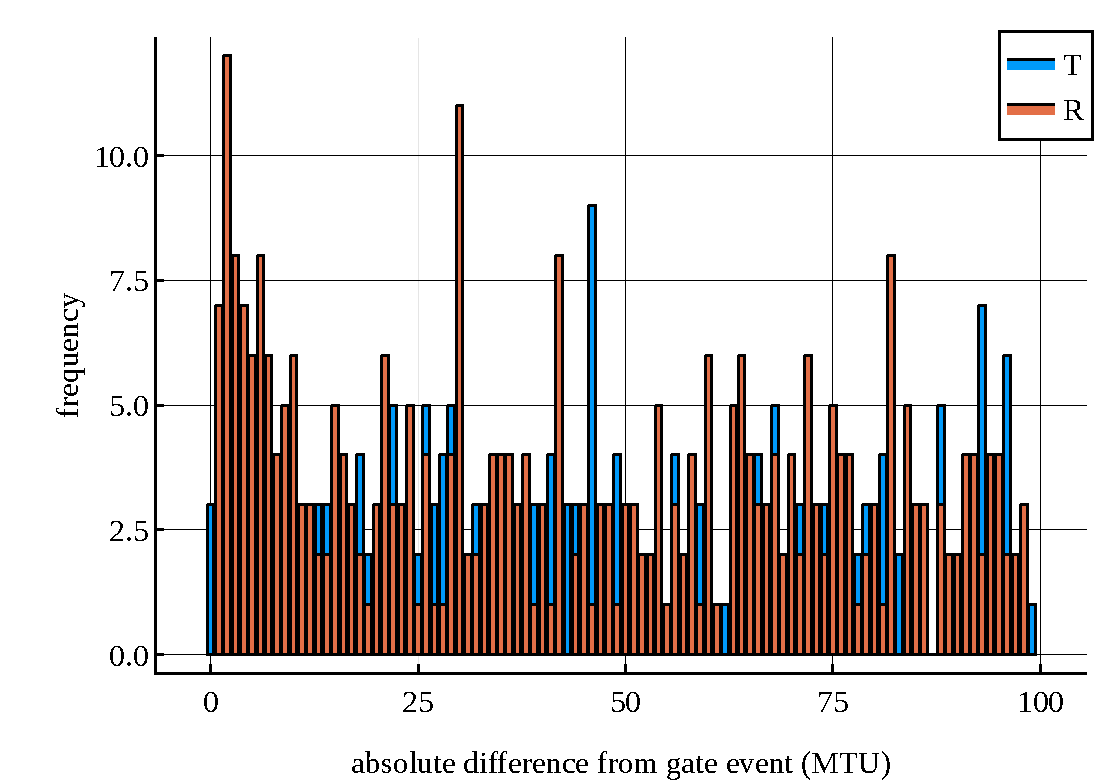
\includegraphics[width = \textwidth]{../images/before.pdf}
            \caption{T, R events before trigger}
            \label{before}
        \end{subfigure}

        \begin{subfigure}{\textwidth}
            \centering
            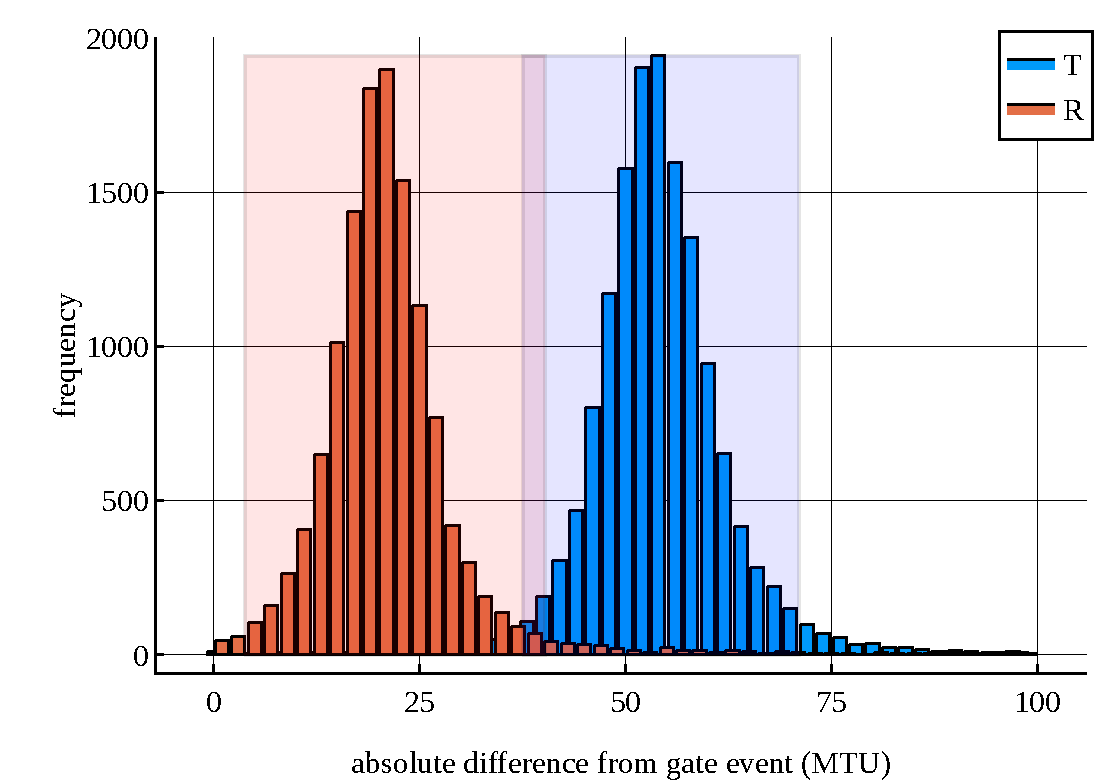
\includegraphics[width = \textwidth]{../images/after.pdf}
            \caption{T, R events after trigger}
            \label{after}
        \end{subfigure}
        \caption{Analysis of inter-channel delay}
    \end{figure}
\end{mdframed}
So we deduce that, in mean, the significant events in the channel $R$ follow the gate event by $\approx 22 MTU$ , and the ones in the $T$ channel follow the gate event by $\approx 54 MTU$.
In conclusion, using the hypotesis that the differential delay is approximatively normally distributed (which can be justified using the Central Limit Theorem), the standard deviations for each bell can be computed using the sample variance, and therefore the \emph{gate} signal is tailored to be a \emph{window} centered in the mean, and of width equal to a desired number of standard deviation, which, in this case, is choosen to be 2. That windows are shown in Figure \ref{after}, and are of the form $[(t_{Gi} + \mu) -2\sigma; \; (t_{Gi} + \mu) + 2\sigma]$ where $t_{Gi}$ is the time of the $i$-th gate event. Using the $\pm 2 \sigma$ interval, we expect to include in that way the $95\%$ of events. This construction of the gate window  considers all the event belonging to the external of the windows as \emph{noise}.  

\subsection*{Interpretation of results and conclusions}
By filtering the events with the gate function described in the previous paragraph, we are able to measure the realization frequencies associated to the random variables $X_r, \, X_t$. The results are shown in Table \ref{result}, along with estimated errors.
In order to compute the errors, the sample variance is used to deduce the standard deviation $\sigma_{p}$. For a Bernoulli random variable of estimated probability $p$ it is calculated as
\begin{equation*}
    \sigma_{p} = \sqrt{\frac{p(1-p)}{N_1-1}}
\end{equation*}
using the Bessel correction at the denominator.

As for the error in $\hat{\alpha}$, a similar estimate is not readily applicable, as there is no trivial probabilistic description of this estimator. However, a basic error propagation estimate, using Taylor series, is carried out using the standard deviations of the probabilities as errors to be propagated. 
\renewcommand{\arraystretch}{1.5}
\begin{mdframed}
    \begin{table}[H]
        \centering
        \begin{tabular}{|c|c|c|}
            \hline
            $p_t$ & $0.5130 \pm 0.003017$\\
            \hline
            $p_r$ & $0.4871 \pm 0.003017$\\
            \hline
            $p_c$ & $(3.6429 \pm 3.6429) \cdot 10^{-5}$\\
            \hline
            $\alpha$ & $(1.458  \pm 1.476) \cdot 10^{-4}$\\
            \hline
        \end{tabular}
        \caption{Estimates of probabilites and correlation from data}
        \label{result}
    \end{table}
\end{mdframed}
It may seem a problem that the estimated errors on $p_c$ and $\alpha$ are so large to be comparable to the actual magnitudes, but this is due to the poor statistics of the sample of triple coincidences: in fact, only 1 over 27451 gate events leads to a triple coincidence, and this greatly compromises the accuracy of the probability estimations. 

Nonetheless this great uncertainty \emph{does not invalidate the physical conclusion}: this value of $\alpha$ shows a near-perfect anticorrelation, and is in complete contradiction with respect to the classical theory. 


\begin{mdframed}
    \begin{figure}[H]
        \centering
        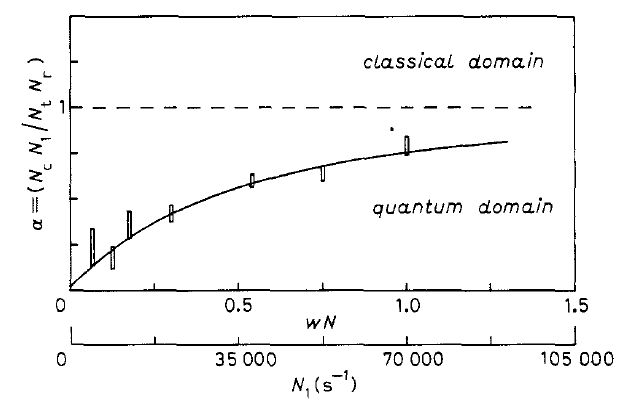
\includegraphics[width = \textwidth]{../images/alpha.png}
        \caption{Original experiment results}
        \label{alpha}
    \end{figure}
\end{mdframed}
In addition, the result on $\alpha$ and it's error seem to be compatible with the result obtained by Grangier et. al. shown in Figure \ref{alpha}. In the horizontal axis there is the average gate trigger rate, which in the case of the collected data, after the filtering,  is $\approx 1 Hz$, so it is extremely low with respect to the order of magnitude of the one of the original experiment. This justifies such a low value of $\alpha$ with respect of the values shown in this plot.

In conclusion, the scope of the experiment is met: this experiment validate the indivisibility of the photons, and, in spite of the classical theory of EM fields, it shows a peculiar quantistic feature of reality. 

\clearpage
\section{Random Number Generation}
In this report two methods of obtaining streams of random bits (i.e. 
 processes of independent and identically distributed Bernoulli $(p = 0.5)$ random variables) are presented.
 Starting from a coherent source of light, the photon arrival times are collected by a time-tagger, so the difference between the arrivals tags represents a realization of a process of i.i.d. exponential random variables. 

 The two methods presented differ mainly in the fact that their algorithms needs different resources: the first one can operate directly on a continuous stream of photon arrivals, whereas the second needs to scan all the sequence of arrivals before generating, in a second scan, the random bits. We will call the first one \emph{Local difference} method, and the second \emph{Median}, for reasons that will be explained in the next paragraphs.
\subsection*{Local difference method}
This algorithm can operate with constant memory over a stream of subsequent time tags, it is ideal for a real-time generation of data from a constantly running optical setup.
The algorithm works as follows:
\begin{enumerate}
    \item generate, from 5 subsequent time tags, a vector of the differences between each one with the previous one, which will be composed of 4 elements, 
    \item group the differences by pairs, and compute a further  difference between the second element of the pair and the first one: a sequence of 2 values $(\Delta_1$, $\Delta_2)$ is obtained,
    \item compare the values: if $\Delta_1 \geq \Delta_2$ set the bit to 1, otherwise set the bit to 0, 
    \item execute 1. to 3. over all the incoming time-tags.
\end{enumerate}
Using the vector of 4353849 time tags belonging to the Arecchi wheel experiment, we generate $\lfloor4353849/(4\cdot 8)\rfloor = 136057$ bytes which represents numbers from 0 to 255.

Using them as triplets of coordinates it is possible to build a 3D scatter plot to show their uniform distribution among space. In Figure \ref{local} this representation, along with and the histogram of frequencies in Figure \ref{loca}.
\begin{mdframed}
    \begin{figure}[H]
            \centering
            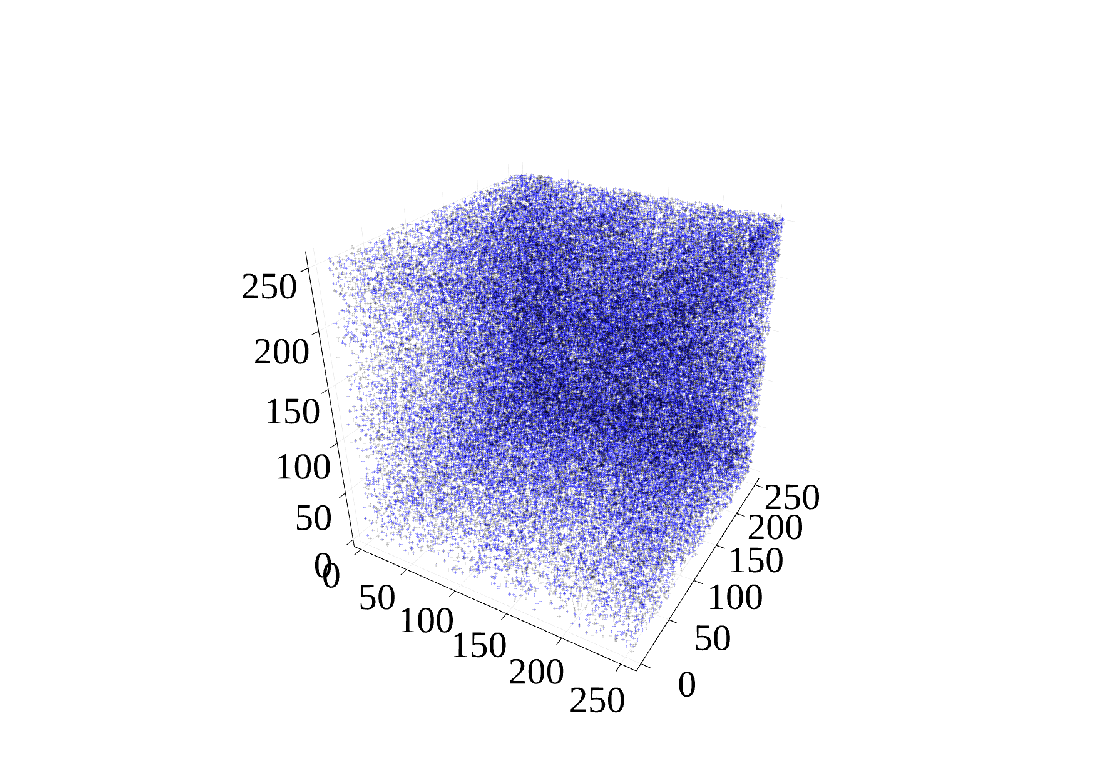
\includegraphics[width = \textwidth]{../random_img/d2-scatter3d.pdf}
            \caption{Local difference method, 3D Scatter}
            \label{loca}
        \end{figure}
    \end{mdframed}
    \begin{mdframed}

        \begin{figure}[H]
            \centering
            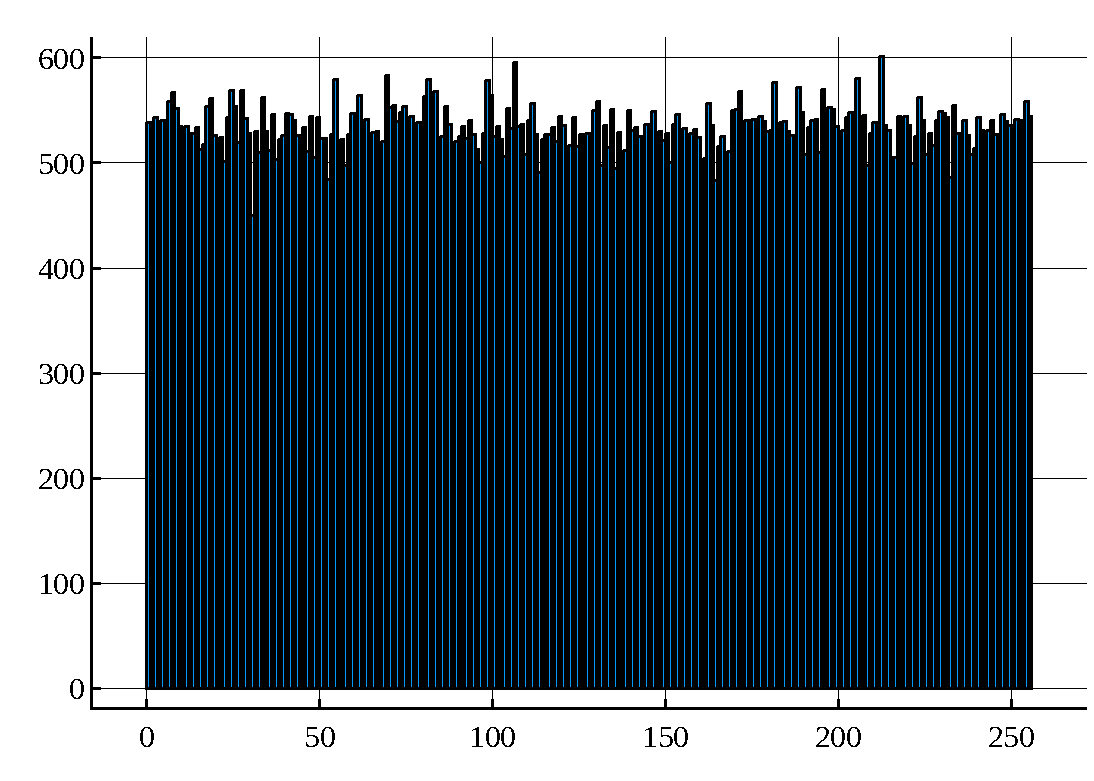
\includegraphics[width = \textwidth]{../random_img/d2-histogram.pdf}
        \caption{Local difference method, histogram}
        \label{local}
    \end{figure}
\end{mdframed}

\subsection*{Median method}
This algorithm can operate with a double examination of the stream of the time tags, the first one is used to deduce the median of the distribution, and the second one exploits a properity of the median to generate the random bits: given a realization from the distribution, it has $50\%$ probability to be above or below the median. We recall that for an exponentially distributed random variable $X \sim Exp(\lambda)$, the median is $\tilde{x} = \ln(2)/\lambda$.
The algorithm works as follows:
\begin{enumerate}
    \item generate from the time tags the vector of the differences between each one with the previous one (skip the first tag),
    \item compute the sample median $\widetilde{d}$ of the differences vector (or alternatively, assuming an exponential distribution, compute the sample mean and obtain the median multiplying it by $\ln(2)$),
    \item for each differences sample $d_i$, set a bit to 1 if $d_i \geq \widetilde{d}$, otherwise set it to 0.
\end{enumerate}
This algorithm provides a generation rate of 4 times the Local difference method rate, at the expense of a greater computing effort, as can be noticed by the plots in Figure \ref{median}, where there are $\lfloor 4353849/8\rfloor = 544231$ bytes.
\begin{mdframed}
    \begin{figure}[H]
        \begin{subfigure}{\textwidth}
            \centering
            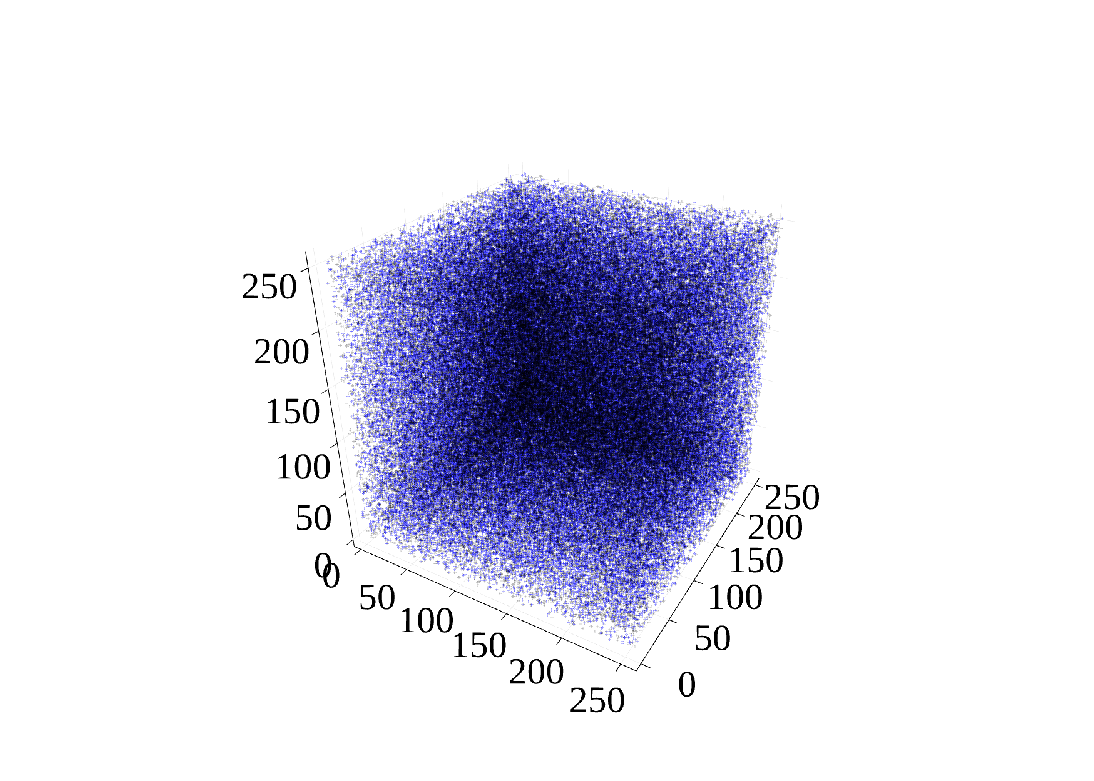
\includegraphics[width = \textwidth]{../random_img/naif-scatter3d.pdf}
            \caption{Scatter 3D}
        \end{subfigure}

        \begin{subfigure}{\textwidth}
            \centering
            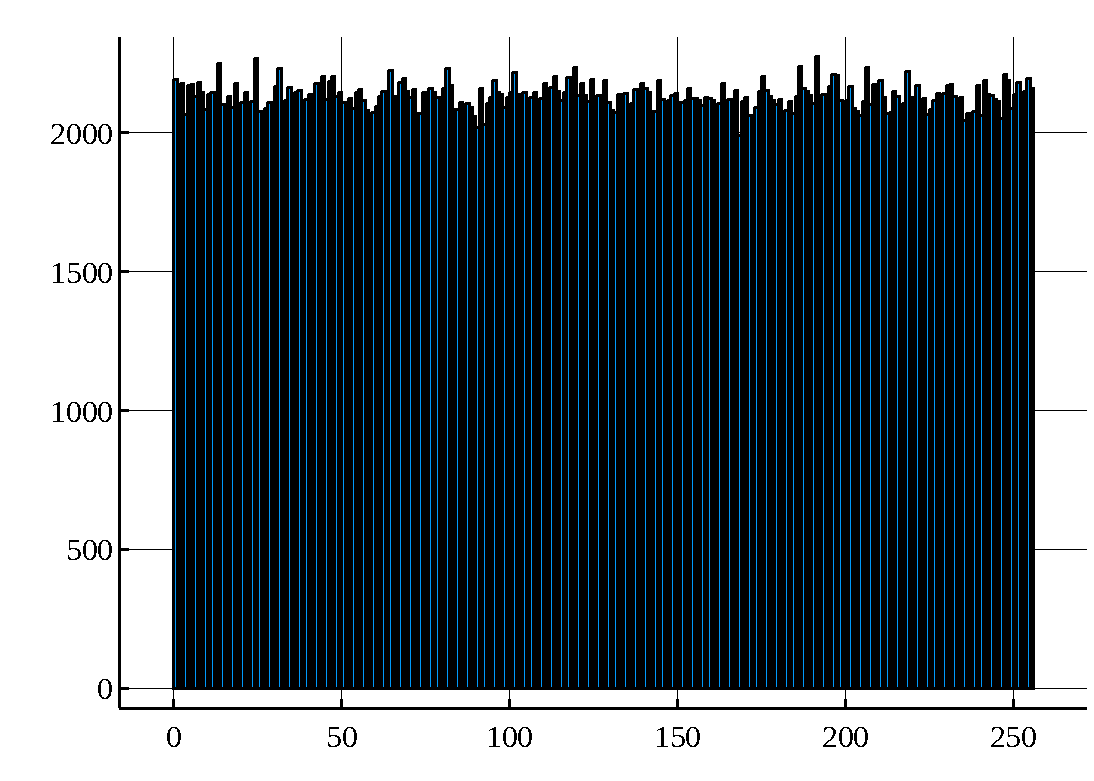
\includegraphics[width = \textwidth]{../random_img/naif-histogram.pdf}
            \caption{Histogram}
        \end{subfigure}
        \caption{Median method}
        \label{median}
    \end{figure}
\end{mdframed}


\subsection*{An even higher efficiency proposal}
If a complete statistical description of the exponential interarrival time process is provided, a much higher rate method is easily developed: using a simple argument on functions of random variables, it can be shown that, if the random variable describing the process is $X \sim Exp(\lambda)$, with cumulative distribution function 
\begin{equation}\label{ewn}
    F_X(x) = 1-\exp[-\lambda x]
\end{equation} 
the variable $Y = F_X(X)$ is uniform in the $[0, 1]$ interval. Once we have obtained that new variable, we can divide the interval $[0, 1]$ in, for example, $256$ even sections, and consider, for each interarrival time value, the $8$-bit number corresponding to the section in which it's transformed value will fall. Each of these sections is equiprobable, so we expect to generate a uniform distribution of $8$-bit numbers. 

The efficiency with respect to the median method can be scaled in this way of a factor of $8$ or higher.
However, this method is of difficult implementation, as it suffers from the  statistical description of the incoming process, which can only be estimated, and from the not perfect time resolution of the time-tagger, that saves the events in a fundamentally discrete space of time tags. It also needs an additional step for each interarrival time to be transformed as equation (\ref{ewn}) indicates.

\hrulefill 
\bibliography{References}
\begin{thebibliography}{99}
  \bibitem{grangier} P.Grangier, G.Roger, A.Aspect - \emph{Experimental evidence for a photon anticorrelation effects on a beam splitter: a new light on single-photon interferences} (Europhys. Lett., 1 (4), pp. 173-179, 1986)
  \bibitem{hc} R.V.Hogg, J.W.McKean, A.T.Craig, \emph{Introduction to mathematical statistics} (Pearson, 2019)
\end{thebibliography}
\end{multicols}



\clearpage
\subsection*{Code}
The code is written in Julia Programming Language.

1. Analysis of photon indivisibility experiment
\renewcommand{\baselinestretch}{0.5}
\begin{mdframed}
    \begin{lstlisting}
module Analyzer
using Plots
using Printf
import Plotly
import PGFPlots
import Statistics
import ProgressMeter

export delay_estimator, loader, difference_info, gated_counter, single_chan_stat, config

default(show = true)
const machine_time = 80.955e-12

function loader(;aft_filter = true)
    println("Loading...")
    s = "./tags.txt"
    a = readlines(s)
    for y in a
        filter(x -> !isspace(x), y)
    end
    i=0
    b = Array{Int, 2}(undef, 2, length(a))

    b[1, :] = [parse(Int, split(x, ";")[1]) for x in a]
    b[2, :] = [parse(Int, split(x, ";")[2]) for x in a]


    tags = Array{Int, 2}(undef, 3, length(b))
    fill!(tags, 0)
    println(typeof(tags))
    k = Array{Int, 1}(undef, 3) # k[i] will be the total count of trigger events on channel i
    fill!(k, 1)
    i=0
    cnt = 0
    aft = Array{Int, 1}(undef, 3)
    fill!(aft, 0)
    if (aft_filter)
        aft_const = 3900
    else
        aft_const = 0
    end
    for i = 1:length(a)
         if (i<8 || tags[ b[2, i]-1, k[b[2, i]-1] - 1 ] + aft_const < b[1, i] )
            tags[ b[2, i]-1, k[b[2, i]-1] ] = b[1, i]
            k[b[2, i] - 1] += 1
        else
            aft[b[2, i] - 1] +=1
        end
    end

    println("Number of valid hits")
    @printf("\t n. of transmitted hits   : %6d \n", k[1])
    @printf("\t n. of reflected hits     : %6d \n", k[2])
    @printf("\t n. of gate hits          : %6d \n", k[3])
    println("T+R = ", k[1]+k[2], ", G = ", k[3])
    println("Number of afterpulses:")
    @printf("\t chan 1 - transmitted (2) : %6d \n", aft[1])
    @printf("\t chan 2 - reflected (3)   : %6d \n", aft[2])
    @printf("\t chan 3 - gate (4)        : %6d \n", aft[3])
    println("Percentage of afterpulses")
    @printf("\t chan 1 - transmitted (2) : %4.1f %% \n", aft[1]/k[1] * 100)
    @printf("\t chan 2 - reflected (3)   : %4.1f %% \n", aft[2]/k[2] * 100)
    @printf("\t chan 3 - gate (4)        : %4.1f %% \n", aft[3]/k[3] * 100)
    return (tags, k);
end

function delay_estimator((tags, k); mode = "gate_first")
    println("Analyzing...")
    machine_time = 80.955e-12
    diff1 = Array{Int, 1}(undef, k[1])
    diff2 = Array{Int, 1}(undef, k[2])
    fill!(diff1, 0)
    fill!(diff2, 0)
    if mode == "gate_last"
        g1 = -1
        g2 = tags[3, 1]
        n = 1
        # Retarded gate method - positive diff
        for i = 2:k[3]
            while (tags[1, n]<g2 && n<k[1])
                diff1[n] = g2 - tags[1, n]
                n += 1
            end
            g2 = tags[3, i]
        end

        g1 = -1
        g2 = tags[3, 1]
        n = 1
        for i = 2:k[3]
            while (tags[2, n]<g2 && n<k[2])
                diff2[n] = g2 - tags[2, n]
                n += 1
            end
            g2 = tags[3, i]
        end
    elseif mode == "gate_first"
        # Anticipated gate method - positive diff
        g1 = -1
        g2 = tags[3, 1]
        n = 8
        for i = 2:k[3]
            while (tags[1, n]<g2 && n<k[1])
                diff1[n] = tags[1, n] - g1
                n += 1
            end
            g1 = g2
            g2 = tags[3, i]
        end
        diff1 = diff1[8:length(diff1)]

        g1 = -1
        g2 = tags[3, 1]
        n = 8
        for i = 2:k[3]
            while (tags[2, n]<g2 && n<k[1])
                diff2[n] = tags[2, n] - g1
                n += 1
            end
            g1 = g2
            g2 = tags[3, i]
        end
        diff2 = diff2[8:length(diff2)]
    else
        # Minimum distance method
        g1 = -100000000
        g2 = tags[3, 1]
        n = 1
        for i = 2:k[3]
            while (tags[1, n]<g2 && n<k[1])
                if ((tags[1, n] - g1) <  (g2 - tags[1, n]))
                    diff1[n] = tags[1, n] - g1
                else
                    diff1[n] = tags[1, n] - g2
                end
                n += 1
            end
            g1 = g2
            g2 = tags[3, i]
        end
        g1 = -100000000
        g2 = tags[3, 1]
        n = 1
        for i = 2:k[3]
            while (tags[2, n]<g2 && n<k[1])
                if ((tags[2, n] - g1) <  (g2 - tags[2, n]))
                    diff2[n] = tags[2, n] - g1
                else
                    diff2[n] = tags[2, n] - g2
                end
                n += 1
            end
            g1 = g2
            g2 = tags[3, i]
        end
    end
    max_clicks = 100
    max_delay = max_clicks * machine_time / 1e-9
    @printf("PRE-filtering at max delay = %d ns \n ", max_delay)
    filter!(x-> (x< max_clicks), diff1)
    filter!(x-> (x< max_clicks), diff2)
    
    difference_info(diff1, diff2, k)
    mu_1 = Statistics.mean(diff1)
    mu_2 = Statistics.mean(diff2)
    sigma_1 = sqrt(Statistics.var(diff1 .- mu_1))
    sigma_2 = sqrt(Statistics.var(diff2 .- mu_2)) 

    return [mu_1, sigma_1, mu_2, sigma_2]
end

function difference_info(diff1, diff2, k)
    machine_time = 80.955e-12
    println("Difference Info...")
    max_diff1 = maximum(diff1)
    min_diff1 = minimum(diff1)
    max_diff2 = maximum(diff2)
    min_diff2 = minimum(diff2)
    @printf("1) maximum difference      : %10d \n", max_diff1)
    @printf("1) minimum difference      : %10d \n", min_diff1)
    @printf("1) maximum time difference  (ns)  : %10.4f \n", max_diff1 * machine_time * 1e9)
    @printf("1) minimum time difference  (ns)  : %10.4f \n", min_diff1 *machine_time * 1e9)

    @printf("2) maximum difference      : %10d \n", max_diff2)
    @printf("2) minimum difference      : %10d \n", min_diff2)
    @printf("2) maximum time difference  (ns)  : %10.4f \n", max_diff2*machine_time * 1e9)
    @printf("2) minimum time difference  (ns)  : %10.4f \n\n", min_diff2*machine_time * 1e9)

    @printf("1) Fraction of accepted hits : %d / %d = %4.2f \n", length(diff1), k[1], length(diff1)/k[1])
    @printf("2) Fraction of accepted hits : %d / %d = %4.2f\n", length(diff2), k[2], length(diff2)/k[2])

    mod = Int(ceil(maximum([length(diff1), length(diff2)]) / 1e4))

    # plot clicks 
    x_delays1 = (min_diff1:mod:max_diff1)
    x_delays2 = (min_diff2:mod:max_diff2)

    bin_num1 = Int(floor((max_diff1-min_diff1) / mod)) + 1
    println("bins 1: ", bin_num1)
    bias1 = Int(floor(-min_diff1/mod))
    hist1 = Array{Int, 1}(undef, bin_num1)
    fill!(hist1, 0)
    i = 1
    while (i<=length(diff1))
        hist1[Int(floor((diff1[i] - min_diff1) / mod))+1] += 1
        i += 1
    end

    bin_num2 = Int(floor((max_diff2-min_diff2) / mod)) + 1
    bias2 = Int(floor(-min_diff2/mod))
    println("bins 2: ", bin_num2)
    hist2 = Array{Int, 1}(undef, bin_num2)
    fill!(hist2, 0)
    i = 1
    while (i<=length(diff2))
        hist2[Int(floor((diff2[i] - min_diff2) / mod))+1] += 1
        i += 1
    end
    mu_1 = Statistics.mean(diff1)
    mu_2 = Statistics.mean(diff2)
    sigma_1 = sqrt(Statistics.var(diff1 .- mu_1))
    sigma_2 = sqrt(Statistics.var(diff2 .- mu_2)) 

    if (length(hist1)<600 && length(hist2)<600)
        println("Plotting...")
        # fig = Plotly.figure()
        n_sigma_ = 2
        fig = Plots.bar(x_delays1,
                         hist1,
                         show=true,
                         xlabel = "absolute difference from gate event (MTU)",
                         ylabel = "frequency", 
                         label = "T", 
                         size = (600, 400))
        Plots.bar!(x_delays2, hist2, label = "R")
        rectangle(w, h, x, y) = Plots.Shape(x .+ [0,w,w,0], y .+ [0,0,h,h])

        recr = rectangle(2*n_sigma_*sigma_1, maximum([maximum(hist1), maximum(hist2)]), mu_1-n_sigma_*sigma_1, 0)
        rect = rectangle(2*n_sigma_*sigma_2, maximum([maximum(hist1), maximum(hist2)]), mu_2-n_sigma_*sigma_2, 0)
        # Plots.plot!(recr, linewidth = 2, opacity = 0.1, color=:blue, label=nothing)
        # Plots.plot!(rect, linewidth = 2, opacity = 0.1, color=:red, label=nothing)

        display(fig)
        savefig("./images/delays.pdf")
    else
        println("Too long to plot...")
    end
end

function gated_counter((tags, k), params; mode = "confidence")
    println("Gated counting...")
    mu_1 = params[1]
    sigma_1 = params[2]
    mu_2 = params[3]
    sigma_2 = params[4]

    @printf("mean tramsmitted   : %6.4f \n", params[1])
    @printf("stdd tramsmitted   : %6.4f \n", params[2])
    @printf("mean     reflected : %6.4f \n", params[3])
    @printf("stdd     reflected : %6.4f \n", params[4])
    N_1 = 0
    intervals = [2]
    for n_sigma_ in intervals
        max_clicks = 100
        x = 1
        r_hit = false
        refl = 0
        multiple_refl = 0
        y = 1
        t_hit = false
        tran = 0
        multiple_tran = 0
        coincidences = 0
        if (mode == "confidence") 
            for i=1:length(tags[3, :])-1
                r_hit = false
                t_hit = false  
                while  tags[1, x] < -n_sigma_*sigma_1 + tags[3, i] + mu_1
                    x += 1
                end
                while -n_sigma_*sigma_1 + tags[3, i] + mu_1 <= tags[1, x] < +n_sigma_*sigma_1 + tags[3, i] + mu_1 && tags[1, x] < tags[3, i+1] 
                    t_hit = true
                    x += 1
                end
                if t_hit
                    tran += 1
                end

                while  tags[2, y] < -n_sigma_*sigma_2 + tags[3, i] + mu_2 
                    y += 1
                end
                while -n_sigma_*sigma_2 + tags[3, i] + mu_2 <= tags[2, y] < +n_sigma_*sigma_2 + tags[3, i] + mu_2  && tags[2, y] < tags[3, i+1]
                    r_hit = true
                    y += 1
                end
                if r_hit
                    refl += 1
                end
                if r_hit && t_hit
                    coincidences += 1
                end
                if r_hit || t_hit
                    N_1 += 1
                end
            end
        else
            for i=1:length(tags[3, :])-1
                r_hit = false
                t_hit = false 
                while tags[1, x] < tags[3, i]
                    x += 1
                end
                while tags[3, i] <= tags[1, x] < tags[3, i] + max_clicks
                    t_hit = true
                    x += 1
                end
                if t_hit
                    tran += 1
                end

                while tags[2, y] < tags[3, i]
                    y += 1
                end
                while tags[3, i] <= tags[2, y] < tags[3, i] + max_clicks
                    r_hit = true
                    y += 1
                end
                if r_hit
                    refl += 1
                end
                if r_hit && t_hit
                    coincidences += 1
                end
                if r_hit || t_hit
                    N_1 += 1
                end
            end
        end
        @printf("Measurement with ± sigma_ confidence \n")
        println("sigma = ", n_sigma_)
        prob_refl = refl / N_1
        prob_tran = tran / N_1
        prob_triple = coincidences / N_1
        alpha = prob_triple/ (prob_refl * prob_tran)
        @printf("\t gate         hits :  %9d \n", N_1)
        @printf("\t reflected    hits :  %9d \n", refl)
        @printf("\t transmitted  hits :  %9d \n", tran)
        @printf("\t coincidences hits :  %9d \n", coincidences)
        @printf(" ----------------------\n")
        @printf("\t P[double]         : %9.8f \n", prob_refl + prob_tran - 2 *prob_triple)
        @printf("\t P[triple]         : %9.8f \n", prob_triple)
        @printf("\t Alpha             : %9.8f \n", alpha)

        sigma_r = sqrt(prob_refl*(1-prob_refl)/(N_1-1))
        sigma_t = sqrt(prob_tran*(1-prob_tran)/(N_1-1))
        sigma_c = sqrt(prob_triple*(1-prob_triple)/(N_1-1))
        @printf("p_r variance: %9.8f \n", sigma_r)
        @printf("p_t variance: %9.8f \n", sigma_t)
        @printf("p_c variance: %9.8f \n", sigma_c)
        @printf(" variance: %9.8f \n", sigma_c/(prob_refl*prob_tran) + 
                sigma_r * prob_triple/(prob_refl^2*prob_tran) +
                sigma_t * prob_triple/(prob_refl*prob_tran^2))
    end
end

function config()
    Plots.plotly()
    Plots.default(size=(600, 400), 
    guidefont=("times", 14), 
    legendfont=("times", 14),
    tickfont=("times", 14)
    )
end

function single_chan_stat((tags, k))
    machine_time = 80.955e-12
    bin_num = 1000
    hist = Array{Int, 2}(undef, 3, bin_num)
    fill!(hist, 0)
    bin_step = Array{Int}(undef, 3)
    diff = Array{Int, 2}(undef, 3, maximum(k)-1)
    fill!(diff, 0)
    println(length(tags[3, :]), k)
    maxx = 0
    for chan in [1, 2, 3]
        series = tags[chan, :]
        for i = 1:k[chan]-1
            diff[chan, i] = series[i+1] - series[i]
        end
        filter!(z -> (z>0), diff[chan, :])
        max_diff = maximum(diff[chan, :])
        if max_diff>maxx
            maxx = max_diff
        end
    end
    x_axis = 0:bin_num:maxx
    bin_size = maxx/bin_num
    i = 1
    for chan = [1, 2, 3]
        filter!(z -> (z>0), diff[chan, :])
        for i = 1:k[chan]-2
            hist[chan, Int(ceil(diff[chan, i]/bin_size))] += 1
        end
    end

    fig = Plots.plot((0:bin_num-1)*bin_size,
                     [log10(x) for x in hist[1, :]] ,
                     label = string("trasmitted channel"),
                     show=true,
                     xlabel = "Interarrival time (MTU)",
                     ylabel = "Frequency (log)",
                     size = (600, 400))

    Plots.plot!((0:bin_num-1)*bin_size,
                [log10(x) for x in hist[2, :]],
                label = string("reflected channel"))

    Plots.plot!((0:bin_num-1)*bin_size,
                [log10(x) for x in hist[3, :]],
                label = string("gate channel"))
    @printf("Sum 1 : %5.4f \n", sum(hist[1, :]/sum(hist[1, :])))
    @printf("Sum 2 : %5.4f \n", sum(hist[2, :]/sum(hist[2, :])))
    @printf("Sum 3 : %5.4f \n", sum(hist[3, :]/sum(hist[3, :])))

    savefig(string("./images/single_chan.pdf"))
end

end
    \end{lstlisting}
\end{mdframed}

2. Functions involved in generation and analysis of random data
\begin{mdframed}
    \begin{lstlisting}
    function random(tags; mode="naif")
    data = diff(tags[1])
    data_diff = diff(data)[1:2:length(data)]
    println("Generating with ", mode, " rule, over ", length(tags[1]) , " tags stream...")
    println("Diffs length: ", length(data), " \nDiffs_of_diffs length: ", length(data_diff))
    mu =  Statistics.mean(data)
    lambda = 1/mu
    median = Statistics.median(data)
    sigma = sqrt(Statistics.var(data))
    byte_stream = Array{UInt8}(undef, Int(floor(length(data)/8))-1)
    if mode == "naif"
        stream = BitArray(undef, length(data))
        for i = 1:length(data)
            if data[i]<median
                stream[i] = 1
            else
                stream[i] = 0
            end
        end
        byte_stream = Array{UInt8}(undef, Int(floor(length(stream)/8)))
        for i = 1:length(byte_stream)-1
            byte_stream[i] = 
            1*stream[8*i]+2*stream[8*i+1]+4*stream[8*i+2]+8*stream[8*i+3]+
            16*stream[8*i+4]+32*stream[8*i+5]+64*s[8*i+6]+128*stream[8*i+7]
        end
    elseif mode == "high-rate"
        uniform_events = Array{Float64}(undef, length(data)) 
        for i = 1:length(data)
            uniform_events[i] = exp(-data[i] * lambda) - 1
        end

        byte_stream = Array{UInt8}(undef, length(data))
        for i = 1:length(byte_stream)
            byte_stream[i] = -Int(floor(255 * uniform_events[i]))
        end
    elseif mode == "diff"
        stream = BitArray(undef, length(data_diff))
        for i =1:length(data_diff)-1
            if data_diff[i]<data_diff[i+1]
                stream[i] = 1
            else
                stream[i] = 0
            end
        end
        byte_stream = Array{UInt8}(undef, Int(ceil(length(stream)/8)))
        for i = 1:length(byte_stream)-1
            byte_stream[i] = 
            1*stream[8*i]+2*stream[8*i+1]+4*stream[8*i+2]+8*stream[8*i+3]+
            16*stream[8*i+4]+32*stream[8*i+5]+64*s[8*i+6]+128*stream[8*i+7]
        end
    elseif mode == "diff-2"
        stream = BitArray(undef, Int(ceil(length(data_diff))/2))
        fill!(stream, 0)
        k = 1
        for i =1:2:length(data_diff)-2
            if data_diff[i]<data_diff[i+1]
                stream[k] = 1
            else
                stream[k] = 0
            end
            k+=1
        end
        byte_stream = Array{UInt8}(undef, Int(ceil(length(stream)/8)))
        fill!(byte_stream, 0)
        for i = 1:length(byte_stream)-1
            byte_stream[i] = 
            1*stream[8*i]+2*stream[8*i+1]+4*stream[8*i+2]+8*stream[8*i+3]+
            16*stream[8*i+4]+32*stream[8*i+5]+64*s[8*i+6]+128*stream[8*i+7]
        end
    end
    println("Byte stream generated")
    println("mean: ", Statistics.mean(byte_stream))

    rnd_tester(byte_stream)
    return byte_stream
end

function rnd_tester(byte_stream)
    samples = length(byte_stream)-9
    while samples % 3 != 0
        samples -= 1
    end
    println("Analyzing ", samples, " UInt8 numbers...")
    # 3D Scatter
    fig1 = Plots.scatter3d(byte_stream[1:3:samples], byte_stream[2:3:samples], byte_stream[3:3:samples], 
                           markercolor = :blue,
                           markershape = :cross,
                           markersize  = 0.5,
                           opacity = 0.1,
                           label= nothing,
                           tickfont=("times", 12),
                           size = (1024, 768)
                           )  
    # Histogram
    fig2 = Plots.histogram(byte_stream, bins = 256, label= nothing)
    # Random walk
    x = Array{Float64}(undef, samples)
    fill!(x, 0)
    mu = Statistics.mean(byte_stream)
    println("Statistical mean of byte_stream: ", mu)
    for i=2:samples
        x[i] = x[i-1] + byte_stream[i] - 127.5
    end
    fig3 = Plots.plot(1:samples, x, label= nothing, size = (1024, 768))

    display(fig1)
    savefig(fig1, "./random_img/scatter3d.pdf")
    display(fig2)
    savefig(fig2, "./random_img/histogram.pdf")
    display(fig3)
    savefig(fig3, "./random_img/random_walk.pdf")
end
    \end{lstlisting}
\end{mdframed} 
\end{document}